\documentclass[12pt]{article}

\usepackage{graphicx}
\usepackage{booktabs}
\usepackage{geometry}
\usepackage{float}

\geometry{a4paper, margin=1in}

\title{MLflow Experiment Tracking Report}
\author{Student ID: 202201857}
\date{\today}

\begin{document}

\maketitle

\section{Introduction}

This report presents the results of five experiment runs tracked using MLflow. 
Different hyperparameter configurations were explored to evaluate their impact 
on the model performance. The main evaluation metric used for comparison was 
\textbf{Discriminator Accuracy (D\_accuracy)}.

\section{Table View}

Table \ref{tab:runs} shows the five experiment runs sorted by the primary 
performance metric (Discriminator Accuracy).

\begin{table}[H]
\centering
\begin{tabular}{lcccc}
\toprule
Run Name & Accuracy & Loss\_D & Loss\_G & Epochs \\
\midrule
industrious-stag-292 & 1.0000 & 0.0000 & 100.0000 & 10 \\
worried-chimp-726 & 0.9881 & 0.1608 & 4.9441 & 10 \\
merciful-dove-458 & 0.9881 & 0.0771 & 6.2270 & 10 \\
agreeable-seal-312 & 0.9762 & 0.2714 & 5.8024 & 10 \\
marvelous-calf-919 & 0.9524 & 0.2208 & 7.8582 & 10 \\
\bottomrule
\end{tabular}
\caption{Experiment runs sorted by Discriminator Accuracy}
\label{tab:runs}
\end{table}

Figure \ref{fig:tableview} shows the MLflow table view used to compare runs.

\begin{figure}[H]
\centering
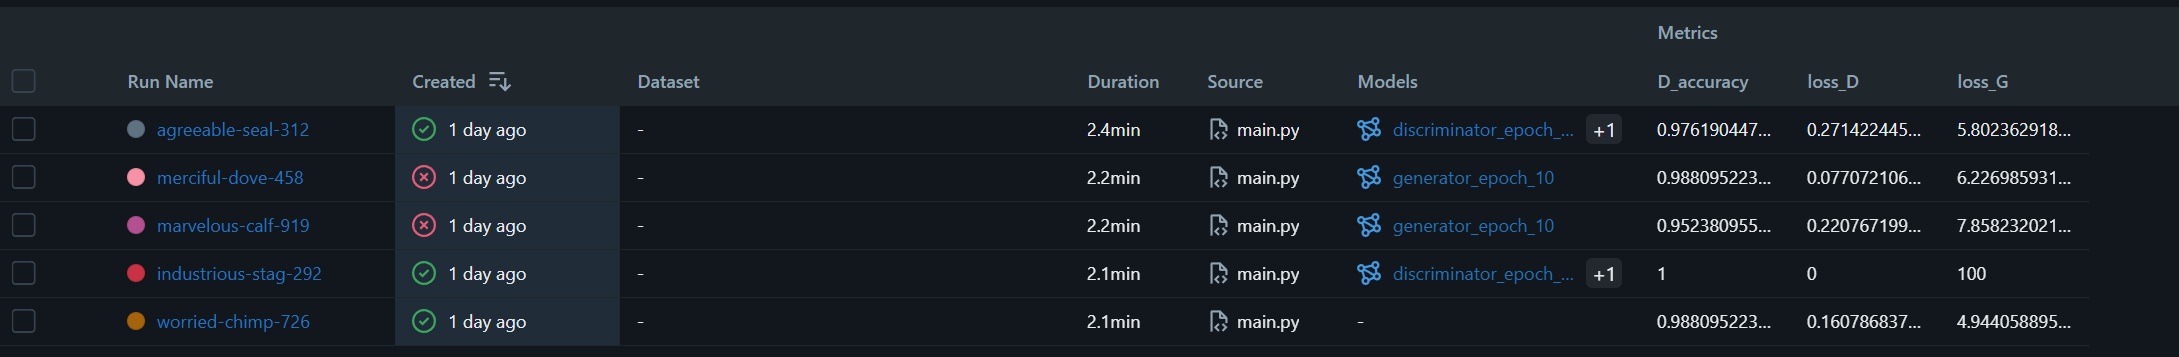
\includegraphics[width=0.9\textwidth]{table_view.png}
\caption{MLflow Table View of experiment runs}
\label{fig:tableview}
\end{figure}

\section{Comparison View}

To better understand the training behavior, multiple runs were selected and 
their performance curves were overlaid using the MLflow comparison tool. 
The accuracy and loss curves help visualize convergence behavior and 
training stability.

Figure \ref{fig:comparison} shows the comparison of at least three runs.

\begin{figure}[H]
\centering
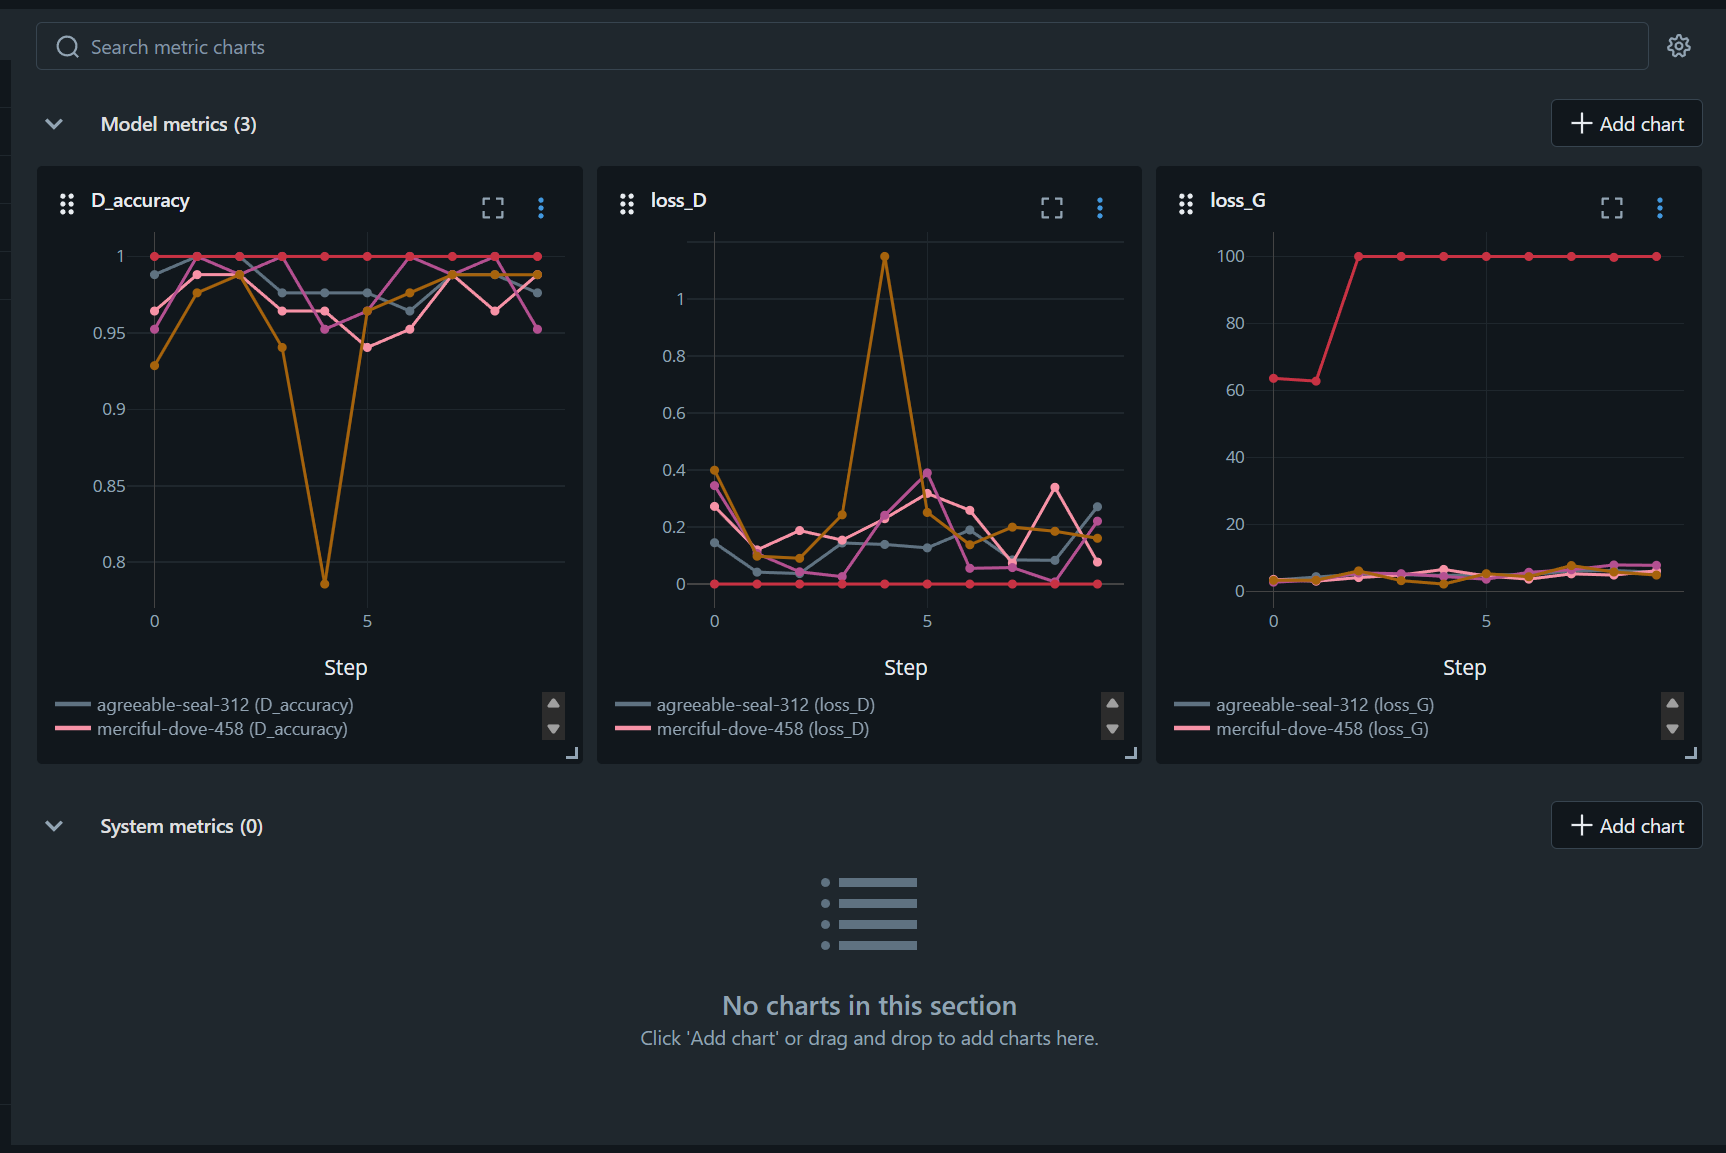
\includegraphics[width=0.9\textwidth]{comparison_view.png}
\caption{Overlayed training curves of multiple runs}
\label{fig:comparison}
\end{figure}

\section{Artifact Gallery}

MLflow automatically logs several artifacts generated during the experiment. 
These artifacts include the trained model and metadata describing the model 
environment.

The artifact gallery includes:

\begin{itemize}
\item The saved trained model
\item The \texttt{MLmodel} metadata file
\item The automatically generated environment files
\end{itemize}

Figure \ref{fig:artifacts} shows the artifacts tab in MLflow.

\begin{figure}[H]
\centering
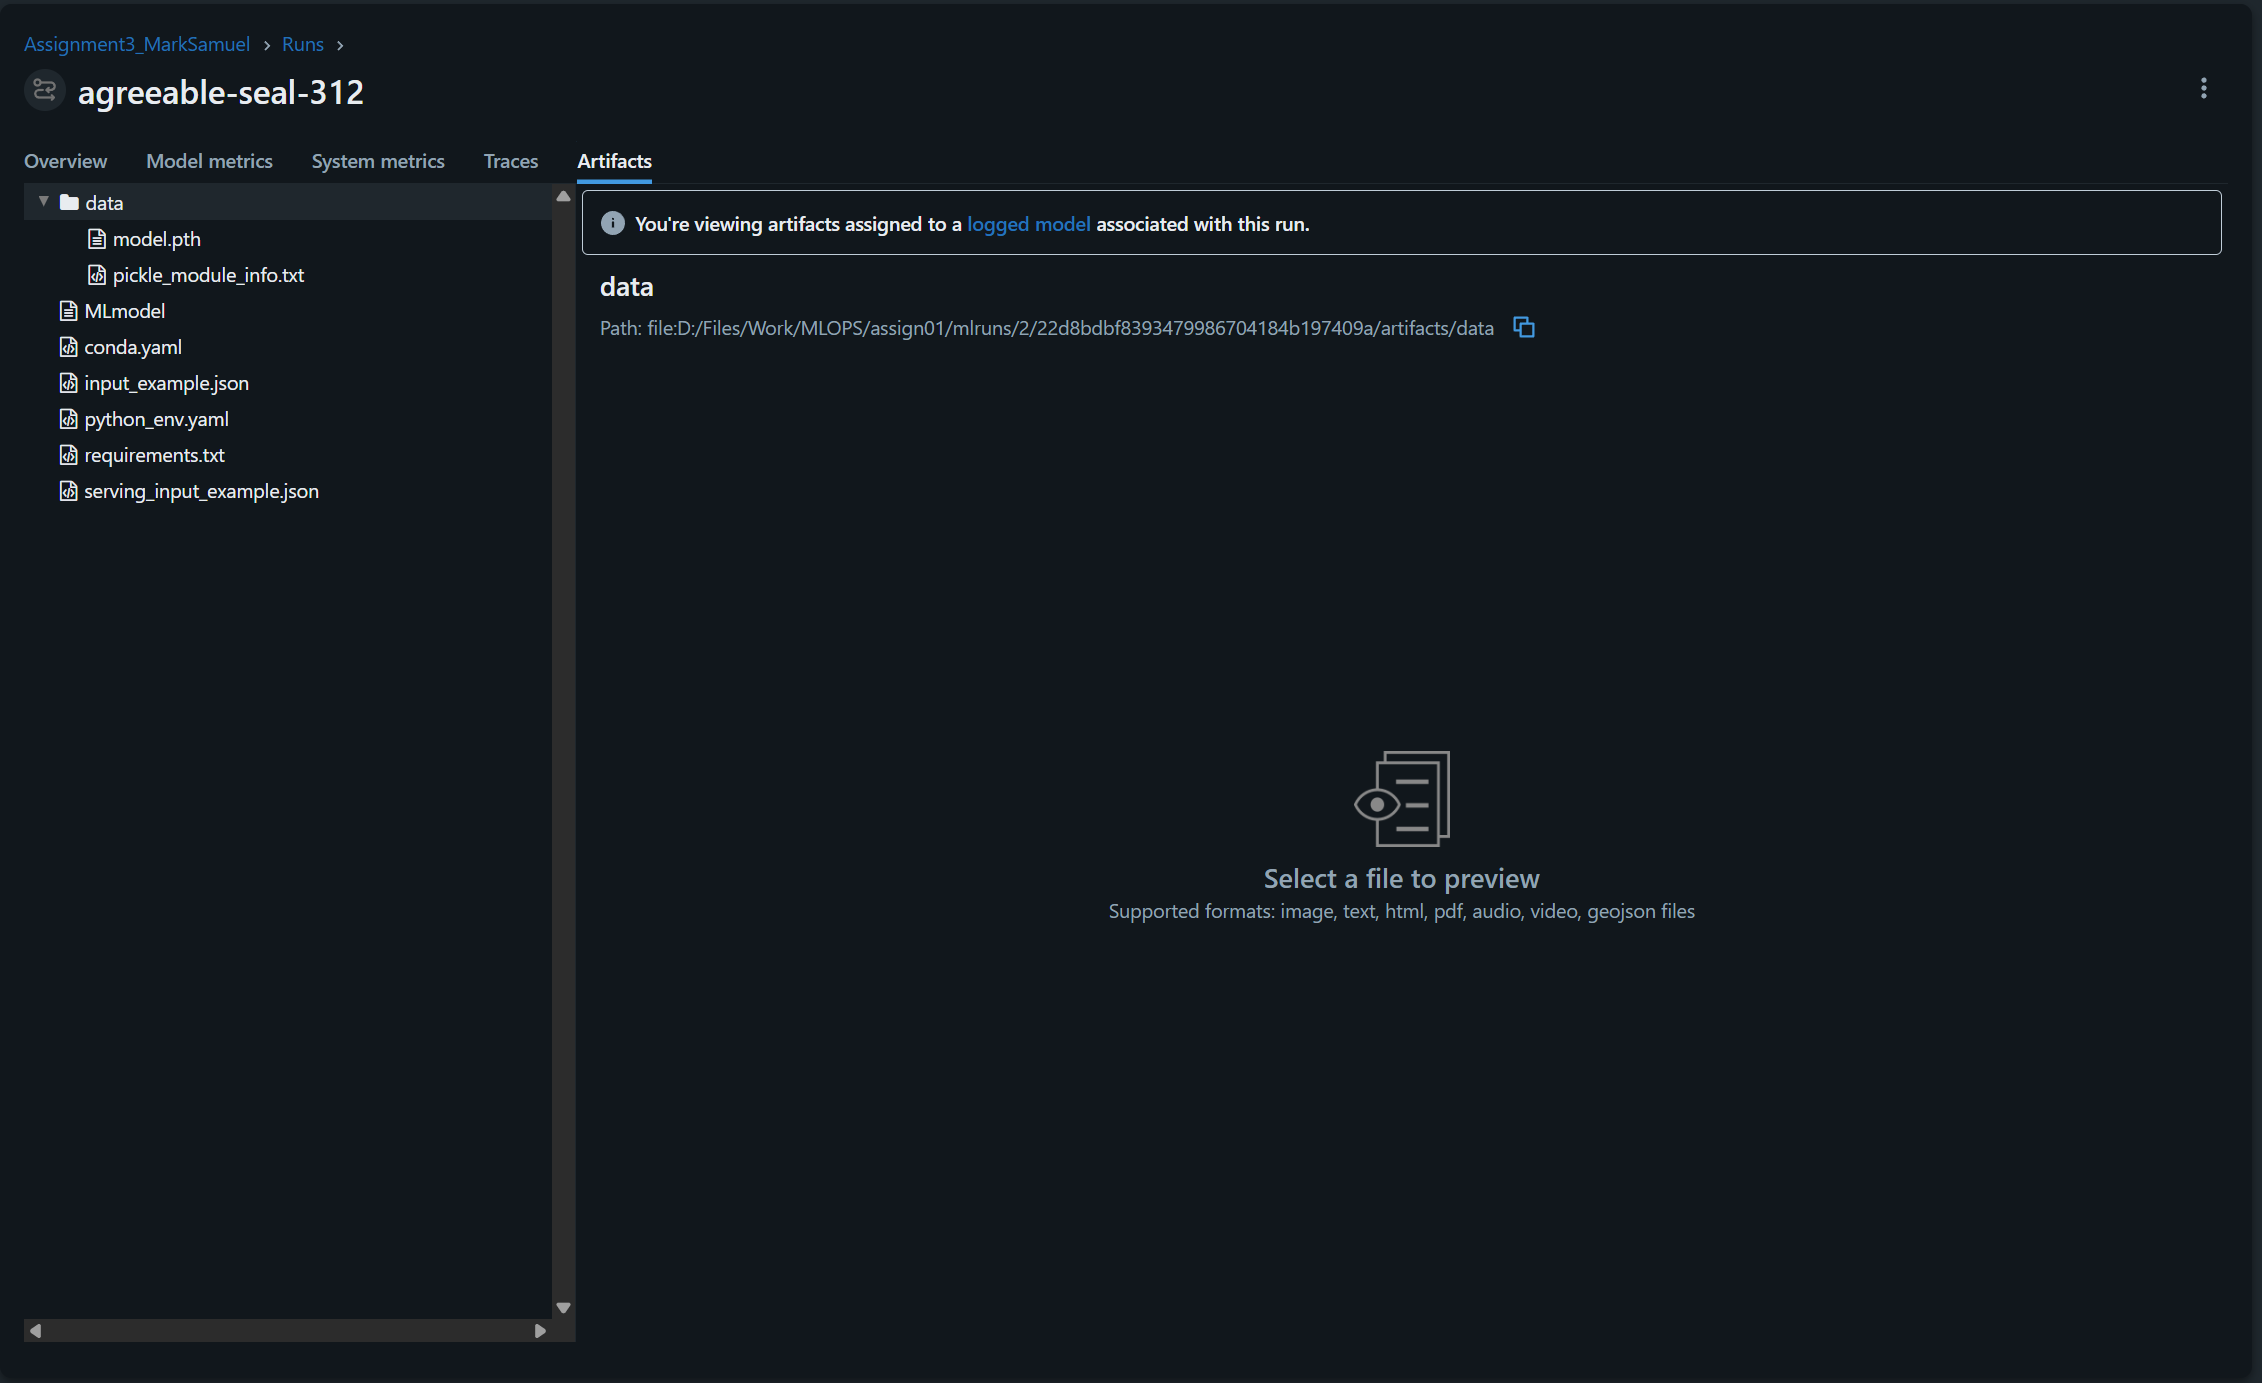
\includegraphics[width=0.9\textwidth]{artifacts.png}
\caption{MLflow Artifact Gallery}
\label{fig:artifacts}
\end{figure}

\section{Short Analysis}

Among the five runs, the run \textbf{worried-chimp-726} was considered the 
best overall run. Although the run \textbf{industrious-stag-292} achieved a 
perfect accuracy of 1.0, its generator loss reached a very high value 
(\texttt{loss\_G = 100}), which indicates unstable GAN training and possible 
mode collapse.

The run \textbf{worried-chimp-726} achieved a high discriminator accuracy 
(\textbf{0.988}) while maintaining a much lower generator loss compared to 
the perfect accuracy run. This suggests a more balanced training process 
between the generator and discriminator.

From the comparison curves, we can observe signs of:

\begin{itemize}
\item \textbf{Overfitting}: Runs where discriminator accuracy quickly 
approaches 1.0 while generator loss grows very large.
\item \textbf{More stable training}: Runs where both losses remain moderate 
and accuracy improves gradually.
\end{itemize}

Overall, the selected winning run provides the best trade-off between high 
accuracy and stable adversarial training dynamics.

\section{Conclusion}

MLflow proved to be a useful tool for tracking experiments, comparing model 
runs, and storing artifacts. The experiment analysis demonstrated how 
different runs can be compared using metrics, training curves, and saved 
artifacts to determine the most reliable model configuration.

\end{document}